\documentclass[11pt,a4paper]{article}
\usepackage[utf8]{inputenc}
\usepackage[T1]{fontenc}
\usepackage{lmodern}
\usepackage[spanish,es-noquoting]{babel}
\usepackage[margin=2.5cm]{geometry}
\usepackage{microtype}
\usepackage{graphicx}
\usepackage{booktabs}
\usepackage{array}
\usepackage{xcolor}
\usepackage{caption}
\usepackage{subcaption}
\usepackage{float}
\usepackage{listings}
\usepackage{fancyhdr}
\usepackage{amsmath}
\usepackage{tikz}
\usetikzlibrary{arrows.meta,positioning}
\usepackage[colorlinks=true,linkcolor=black,urlcolor=black,citecolor=black]{hyperref}

\definecolor{azul}{RGB}{31,95,168}
\definecolor{gris}{RGB}{245,245,245}
\definecolor{comentario}{RGB}{90,110,90}
\captionsetup{font=small,labelfont=bf,format=hang}
\setlength{\parskip}{0.5em}
\setlength{\parindent}{0pt}
\renewcommand{\arraystretch}{1.15}

\lstset{
  basicstyle=\ttfamily\footnotesize,
  backgroundcolor=\color{gris},
  commentstyle=\color{comentario}\itshape,
  keywordstyle=\color{azul}\bfseries,
  numbers=left, numberstyle=\tiny\color{gray}, numbersep=8pt,
  frame=single, rulecolor=\color{gray!40},
  breaklines=true, columns=fullflexible, keepspaces=true,
  xleftmargin=1.5em, framexleftmargin=1.5em,
  captionpos=b, aboveskip=1em, belowskip=0.5em
}
\renewcommand{\lstlistingname}{Código}

\pagestyle{fancy}
\fancyhf{}
\fancyhead[L]{\small Detección de actividad de plagas en restaurantes}
\fancyhead[R]{\small Informe de avance}
\fancyfoot[C]{\thepage}
\renewcommand{\headrulewidth}{0.3pt}

\begin{document}

%-------------------------------------------------- Portada
\begin{titlepage}
\centering
\vspace*{2.5cm}
{\large Sistemas Digitales y Ensambladores (TIC49024)\par}
\vspace{0.4cm}
{\large Periodo 2026-2\par}
\vspace{2.2cm}
\rule{\textwidth}{0.8pt}\\[0.6cm]
{\LARGE\bfseries Detección de actividad de plagas\\en zonas de riesgo de restaurantes\par}
\vspace{0.4cm}
{\Large Informe de avance: software y montaje físico\par}
\rule{\textwidth}{0.8pt}
\vspace{2.5cm}

{\large\textbf{Integrantes}\par}
\vspace{0.3cm}
{\large Luis Esteban Palacios Aparicio\par}
{\large Juan Diego Pérez González\par}
\vfill
{\large 23 de octubre de 2026\par}
\end{titlepage}

\tableofcontents
\newpage

%-------------------------------------------------- 1
\section{Introducción}

El proyecto propone un nodo de bajo costo que detecta actividad compatible con plagas en zonas de riesgo de un restaurante (cocina, bodega, área de basuras). El nodo combina un sensor de movimiento PIR con una cámara basada en ESP32 (placa GOOUUU ESP32-S3-CAM v1.5), que al detectar movimiento captura imágenes y las envía por WiFi, mediante una petición HTTP POST, a un servidor de procesamiento. El servidor, escrito en Python con Flask y OpenCV, analiza las imágenes por sustracción de fondo y registra los eventos sospechosos.

El sistema detecta actividad por el \emph{tamaño} del objeto en movimiento; no identifica la especie del animal.

Este informe presenta el avance a la fecha en dos frentes: (i) el software, con el servidor de procesamiento, sus pruebas automáticas, una evaluación con imágenes sintéticas y la simulación de la lógica del nodo en Wokwi; y (ii) el montaje físico y la prueba de extremo a extremo con el hardware real. La evaluación cuantitativa de la detección se hizo con imágenes generadas por computador; las capturas reales de la cámara se usaron para verificar el flujo completo (captura, envío y procesamiento), no para medir el desempeño de la detección, y los resultados deben leerse con esa salvedad.

%-------------------------------------------------- 2
\section{Arquitectura del sistema}

La Figura~\ref{fig:arq} resume el flujo de información. Cuando el PIR detecta movimiento, el nodo toma una ráfaga de fotografías y la envía al servidor junto con el nombre de la zona; el servidor mantiene un modelo de fondo independiente por zona, evalúa la última fotografía de la ráfaga y, si encuentra un objeto en movimiento dentro del rango de tamaño esperado, guarda un registro en un archivo CSV y una imagen anotada.

\begin{figure}[H]
\centering
\begin{tikzpicture}[
  caja/.style={draw=azul,thick,rounded corners=3pt,minimum height=1.1cm,minimum width=2.6cm,align=center,font=\small},
  flecha/.style={-{Stealth[length=2.5mm]},thick}]
  \node[caja] (pir) {Sensor PIR};
  \node[caja,right=1.2cm of pir] (cam) {ESP32-S3-CAM\\(GOOUUU v1.5)};
  \node[caja,right=1.2cm of cam] (srv) {Servidor\\Flask + OpenCV};
  \node[caja,right=1.2cm of srv] (log) {Registro\\CSV + imagen};
  \draw[flecha] (pir) -- node[above,font=\scriptsize]{disparo} (cam);
  \draw[flecha] (cam) -- node[above,font=\scriptsize]{HTTP POST} node[below,font=\scriptsize]{WiFi} (srv);
  \draw[flecha] (srv) -- (log);
\end{tikzpicture}
\caption{Arquitectura general del sistema.}
\label{fig:arq}
\end{figure}

%-------------------------------------------------- 3
\section{Avance de software}

\subsection{Servidor de procesamiento (versión 2)}

La primera versión del servidor funcionaba, pero presentaba limitaciones que se identificaron al revisarla y que motivaron una segunda versión. La Tabla~\ref{tab:cambios} resume los cambios.

\begin{table}[H]
\centering
\small
\begin{tabular}{>{\raggedright\arraybackslash}p{2.8cm}>{\raggedright\arraybackslash}p{5.4cm}>{\raggedright\arraybackslash}p{5.6cm}}
\toprule
\textbf{Aspecto} & \textbf{Versión 1} & \textbf{Versión 2} \\
\midrule
Modelo de fondo & Uno solo, compartido entre todas las zonas & Un detector independiente por zona \\
Fotos por disparo & Una; el modelo no tenía fondo con qué comparar & Ráfaga: las primeras entrenan el fondo y la última se evalúa \\
Calentamiento & Se evaluaba desde el primer cuadro & No se evalúa hasta haber visto 5 cuadros de la zona \\
Validación de entradas & El nombre de zona se usaba directamente en el nombre del archivo & Nombre saneado (letras, números, guion; máx. 32) y tamaño máximo de petición \\
Consulta de eventos & No existía & Panel web, \texttt{/events} y \texttt{/health} (prototipo) \\
\bottomrule
\end{tabular}
\caption{Cambios de la versión 2 respecto a la versión 1.}
\label{tab:cambios}
\end{table}

\subsubsection*{Detección por sustracción de fondo}

La detección se basa en el sustractor de fondo MOG2 de OpenCV, que modela cada píxel como una mezcla de gaussianas y marca como primer plano aquellos píxeles cuyo valor se aparta del modelo más allá de un umbral de varianza (\texttt{varThreshold}). Con \texttt{detectShadows} activo, los píxeles que el algoritmo interpreta como sombra se etiquetan con el valor 127, y los de primer plano con 255.

El Código~\ref{lst:detector} muestra el método que evalúa un cuadro. Primero se aplica el sustractor y se conservan solo los píxeles de primer plano (umbral en 200, que descarta las sombras). Luego una erosión elimina el ruido aislado y una dilatación une los fragmentos de un mismo objeto. Por último se extraen los contornos y se aceptan únicamente los que tienen un área entre 150 y 8000 píxeles, rango que descarta motas de ruido (muy pequeñas) y personas u objetos grandes (muy grandes).

\begin{lstlisting}[language=Python,caption={Evaluación de un cuadro en \texttt{DetectorZona} (fragmento de \texttt{servidor\_deteccion\_v2.py}).},label={lst:detector}]
def evaluar(self, frame):
    mascara = self.sustractor.apply(frame)
    self.frames_vistos += 1
    # 255 = primer plano; 127 = sombra (se descarta)
    _, mascara = cv2.threshold(mascara, 200, 255, cv2.THRESH_BINARY)
    mascara = cv2.erode(mascara, None, iterations=1)    # quita ruido aislado
    mascara = cv2.dilate(mascara, None, iterations=2)   # une fragmentos
    contornos, _ = cv2.findContours(
        mascara, cv2.RETR_EXTERNAL, cv2.CHAIN_APPROX_SIMPLE)
    eventos = []
    for c in contornos:
        area = cv2.contourArea(c)
        if self.area_min <= area <= self.area_max:
            x, y, w, h = cv2.boundingRect(c)
            eventos.append({"area_px": int(area), "bbox": [x, y, w, h]})
    return eventos
\end{lstlisting}

Cada zona tiene su propia instancia de \texttt{DetectorZona}, con su sustractor y su contador de cuadros vistos. Así, el fondo de una zona no contamina al de otra, problema que sí aparecía con el modelo único de la versión 1.

\subsubsection*{Recepción de ráfagas}

El nodo envía varias fotografías en una sola petición. El Código~\ref{lst:upload} muestra la lógica del \emph{endpoint} \texttt{/upload}: todas las fotografías menos la última se usan para entrenar el modelo de fondo, y solo la última se evalúa. Mientras la zona no haya visto al menos cinco cuadros, la respuesta es \texttt{calentando} y no se emiten alertas.

\begin{lstlisting}[language=Python,caption={Lógica de la ráfaga en \texttt{/upload} (fragmento).},label={lst:upload}]
det = detector_de(zona)
with det.lock:
    for f in frames[:-1]:
        det.entrenar(f)                       # fondo
    if det.frames_vistos < min_frames_fondo:
        det.entrenar(frames[-1])
        return jsonify({"alerta": False, "estado": "calentando",
                        "frames_vistos": det.frames_vistos})
    anotado, eventos = det.evaluar(frames[-1])  # disparo
\end{lstlisting}

\subsection{Pruebas automáticas}

Se escribieron 17 pruebas con \texttt{pytest} que se ejecutan sobre el servidor mediante el cliente de pruebas de Flask, y todas se aprueban. La Tabla~\ref{tab:pruebas} agrupa lo que verifican.

\begin{table}[H]
\centering
\small
\begin{tabular}{>{\raggedright\arraybackslash}p{4.2cm}>{\raggedright\arraybackslash}p{9.6cm}}
\toprule
\textbf{Grupo} & \textbf{Comportamiento verificado} \\
\midrule
Validación de entradas & Petición sin imagen o con imagen corrupta responde 400; nombres de zona inválidos (\texttt{../../etc}, con espacios, de más de 32 caracteres, vacío) se rechazan. \\
Calentamiento & El primer disparo de una zona no genera alerta. \\
Detección & Un objeto del tamaño de una plaga genera alerta, con registro en el CSV y la imagen anotada. \\
Filtros & Se ignoran las motas menores a 150 px, los objetos mayores a 8000 px y los cambios bruscos de iluminación. \\
Ráfagas y zonas & La ráfaga entrena con las primeras fotos y evalúa la última; alternar zonas con fondos distintos no mezcla sus modelos. \\
Consulta y seguridad & \texttt{/events} y el panel muestran los eventos; no se puede salir del directorio de imágenes mediante \texttt{/snapshots}. \\
\bottomrule
\end{tabular}
\caption{Resumen de las 17 pruebas automáticas.}
\label{tab:pruebas}
\end{table}

\begin{lstlisting}[language=Python,caption={Ejemplo de prueba: un objeto de tamaño de plaga debe generar alerta (fragmento de \texttt{test\_servidor.py}).},label={lst:test}]
def test_detecta_objeto_tamano_plaga_y_registra(cliente, fondo, rng):
    cli, logs = cliente
    _calentar(cli, fondo, rng)                 # 5 cuadros de fondo
    img = escenas.frame_vacio(fondo, rng)
    escenas.agregar_objeto(img, rng, 900)      # objeto de ~900 px
    r = _subir(cli, [img]).get_json()
    assert r["alerta"] is True and 150 <= r["eventos"][0]["area_px"] <= 8000
\end{lstlisting}

\subsection{Evaluación con escenas sintéticas}
\label{sec:eval}

Como aún no hay imágenes reales de la cámara, se generaron escenas sintéticas de $640\times480$ píxeles: un piso con baldosas, ruido de sensor y compresión JPEG, con cinco tipos de disparo (vacía, mota, plaga, objeto grande y cambio de luz). Se compararon la versión 1 y la versión 2 del servidor sobre las mismas escenas, con semilla fija para que el experimento sea reproducible. Se usaron tres configuraciones: v1 con una zona (150 disparos), v1 con dos zonas (300) y v2 con dos zonas y ráfaga de 6 fotos (300).

Se definen, a partir de verdaderos positivos (TP), falsos positivos (FP), falsos negativos (FN) y verdaderos negativos (TN):
\begin{equation*}
\text{recall}=\frac{TP}{TP+FN},\qquad
\text{precisión}=\frac{TP}{TP+FP},\qquad
\text{tasa de falsa alarma}=\frac{FP}{FP+TN}.
\end{equation*}

\begin{table}[H]
\centering
\small
\begin{tabular}{lrrrrccc}
\toprule
\textbf{Configuración} & \textbf{TP} & \textbf{FP} & \textbf{FN} & \textbf{TN} & \textbf{Recall} & \textbf{Precisión} & \textbf{Falsa alarma} \\
\midrule
v1, 1 zona, 1 foto  & 61  & 3  & 2 & 84  & 0.968 & 0.953 & 0.034 \\
v1, 2 zonas, 1 foto & 117 & 11 & 2 & 170 & 0.983 & 0.914 & 0.061 \\
v2, 2 zonas, ráfaga & 119 & 1  & 0 & 180 & 1.000 & 0.992 & 0.006 \\
\bottomrule
\end{tabular}
\caption{Resultados sobre escenas sintéticas (semilla 2026).}
\label{tab:eval}
\end{table}

\begin{figure}[H]
\centering
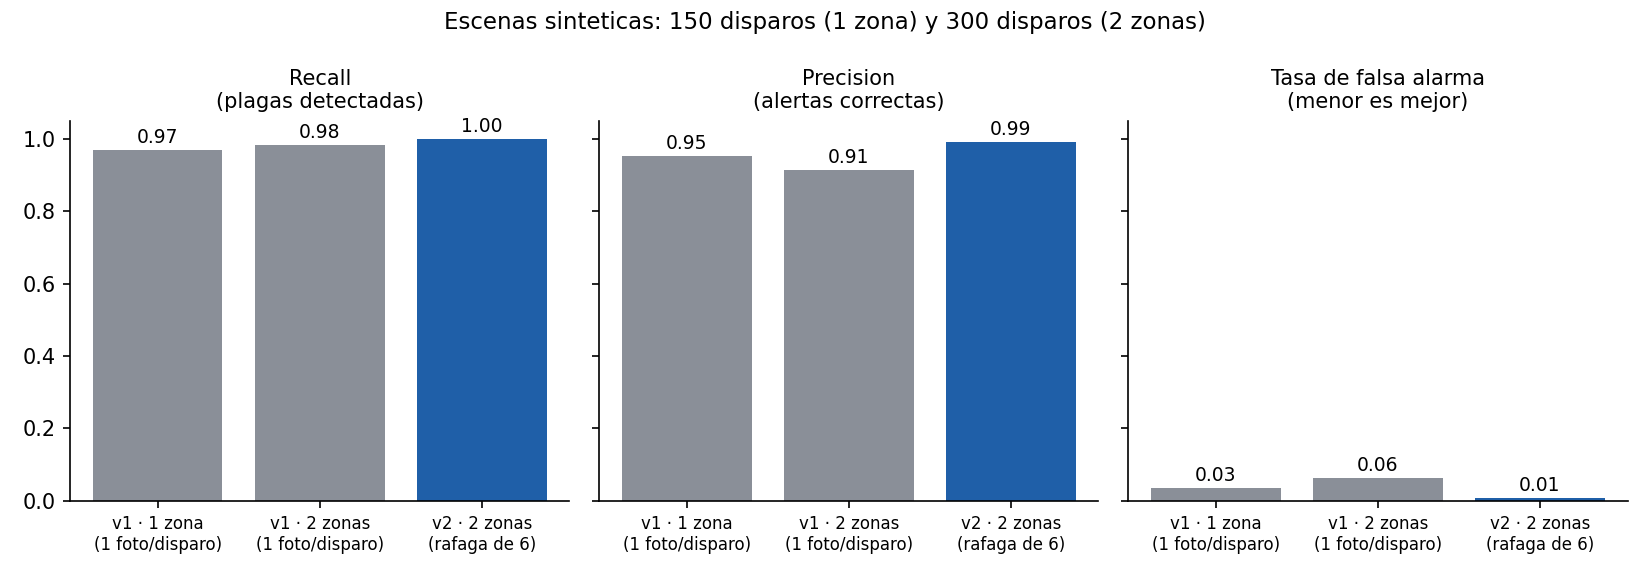
\includegraphics[width=\textwidth]{img/fig1_comparacion.png}
\caption{Comparación entre las versiones 1 y 2 en recall, precisión y tasa de falsa alarma.}
\label{fig:comp}
\end{figure}

La versión 1 ya funcionaba razonablemente con una sola zona (recall de 0.97 y precisión de 0.95). Al pasar a dos zonas empeora: las 11 falsas alarmas corresponden a 5 motas, 5 cambios de luz y 1 objeto grande, consistente con que el modelo compartido se contamina al alternar fondos distintos. La versión 2 reduce las falsas alarmas a una y detecta las 119 plagas simuladas. En tiempo de procesamiento, la v2 tarda unos 15 ms por disparo (6 fotos) frente a unos 2.3 ms de la v1 (1 foto), medido en el computador; es un costo despreciable frente al tiempo de envío por WiFi. Las muestras son pequeñas y sintéticas, de modo que las diferencias pequeñas entre versiones no deben tomarse como definitivas.

\begin{figure}[H]
\centering
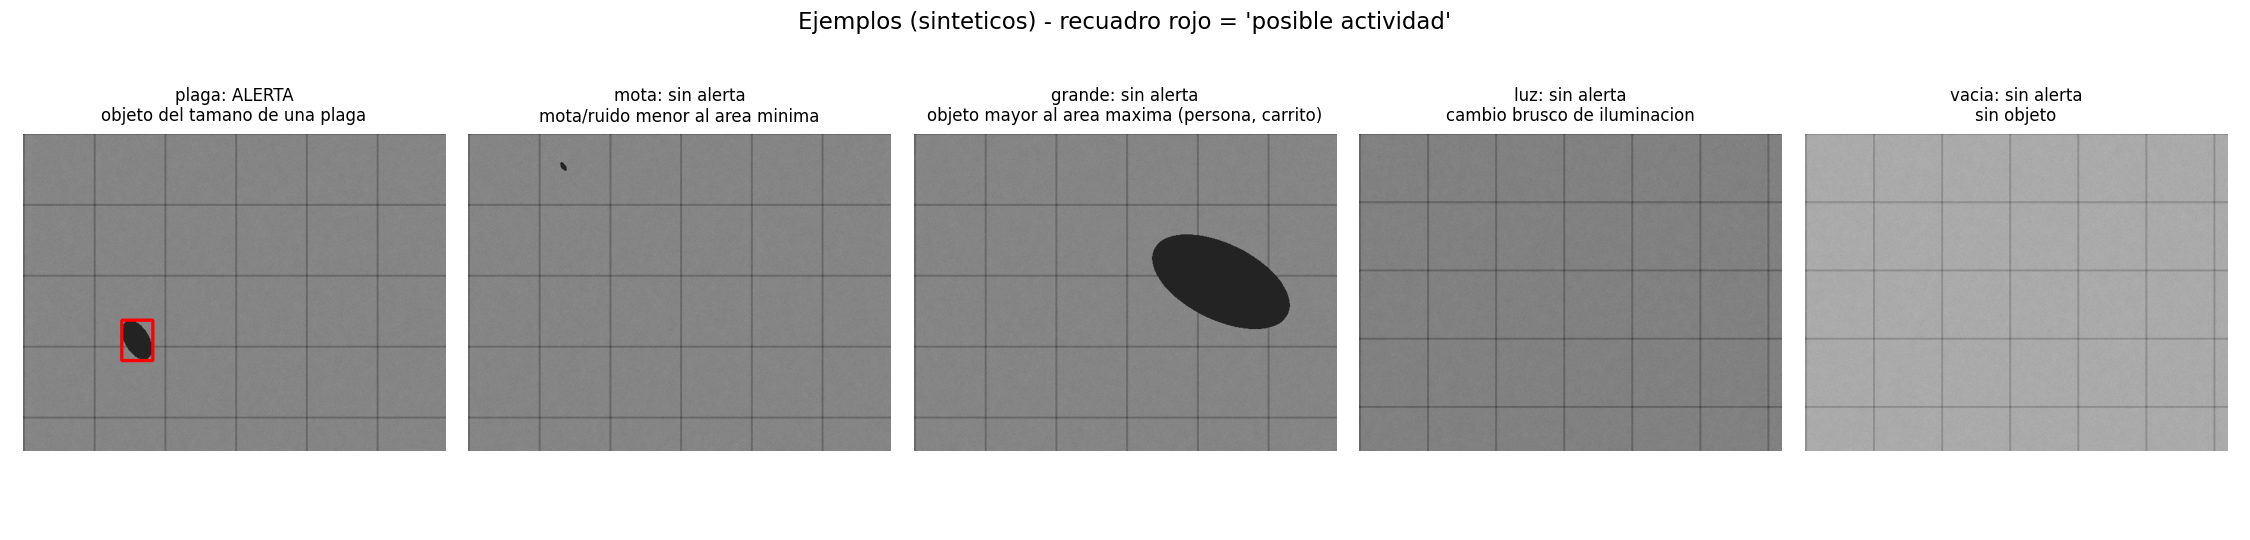
\includegraphics[width=\textwidth]{img/fig2_ejemplos.png}
\caption{Un ejemplo de cada tipo de escena; el recuadro rojo indica posible actividad.}
\label{fig:ejemplos}
\end{figure}

\subsection{Hallazgo de diseño: tamaño mínimo de la ráfaga}

Durante las pruebas se observó que, con cuatro cuadros de fondo o menos, MOG2 clasifica el objeto oscuro como sombra y no lo detecta (0 de 40 casos), mientras que con cinco o más lo detecta siempre (40 de 40), como muestra la Figura~\ref{fig:calent}. Por esta razón el servidor exige cinco cuadros de calentamiento y el firmware debe enviar al menos seis fotografías por disparo del PIR: cinco para el fondo y una para evaluar. El firmware desarrollado (Sección~\ref{sec:fisico}) ya envía ráfagas de seis fotografías. No se profundizó en la causa interna de este comportamiento de MOG2.

\begin{figure}[H]
\centering
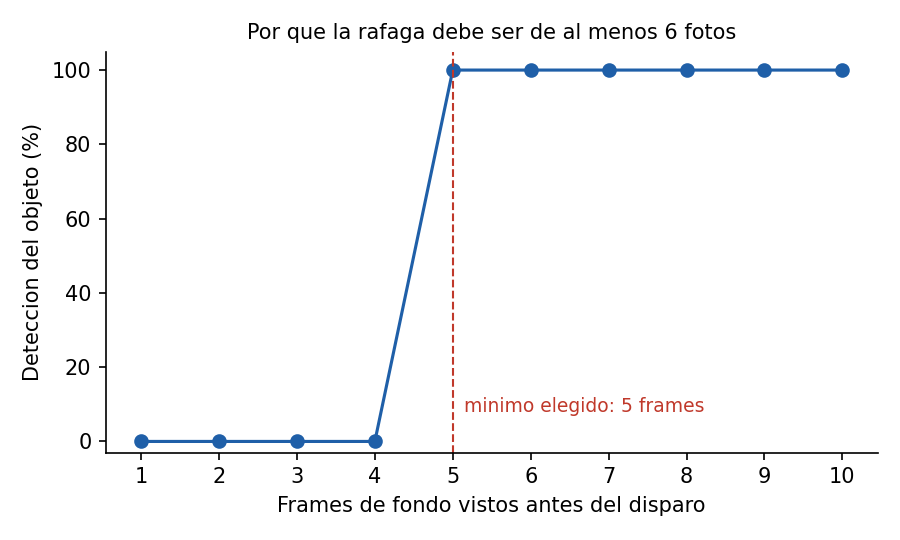
\includegraphics[width=0.62\textwidth]{img/fig3_calentamiento.png}
\caption{Detección de un objeto en función de los cuadros de fondo vistos antes del disparo.}
\label{fig:calent}
\end{figure}

%-------------------------------------------------- 4
\section{Simulación del nodo en Wokwi}

Para validar la lógica de disparo sin depender del hardware, se simuló en Wokwi un ESP32 DevKit (equivalente en lógica a la placa real, ya que Wokwi no incluye la GOOUUU) con un sensor PIR en el GPIO 13 (el mismo pin previsto para el montaje real) y un LED en el GPIO 2 que indica captura en curso. El Código~\ref{lst:wokwi} muestra el ciclo principal: se detecta el flanco de subida del PIR y, si ha pasado el tiempo de enfriamiento de 5 s desde el último disparo, se captura una ráfaga de 6 fotografías separadas 200 ms. El enfriamiento evita disparos repetidos mientras la salida del PIR permanece en alto.

\begin{lstlisting}[language=C++,caption={Ciclo principal de la simulación (fragmento de \texttt{sketch.ino}).},label={lst:wokwi}]
#define PIN_PIR 13
#define FOTOS_POR_RAFAGA 6      // minimo que necesita el servidor v2
#define ENFRIAMIENTO_MS 5000

void loop() {
  bool pir = digitalRead(PIN_PIR) == HIGH;
  bool flancoSubida = pir && !pirAnterior;
  pirAnterior = pir;

  if (flancoSubida && (millis() - ultimoDisparo > ENFRIAMIENTO_MS || disparos == 0)) {
    ultimoDisparo = millis();
    disparos++;
    Serial.printf("[PIR] movimiento detectado (disparo #%d)\n", disparos);
    capturarRafaga();           // 6 fotos, LED encendido durante la captura
  } else if (flancoSubida) {
    Serial.println("[PIR] movimiento ignorado (enfriamiento)");
  }
  delay(20);
}
\end{lstlisting}

En la simulación, el monitor serie muestra el mensaje de inicio, y al activar el sensor aparecen el disparo y las seis capturas, seguidas del aviso de que la ráfaga está lista para enviarse (Figura~\ref{fig:wokwi}). Wokwi no simula la cámara ni el envío HTTP al servidor local, por lo que esta etapa valida únicamente la lógica PIR $\rightarrow$ ráfaga.

\begin{figure}[H]
\centering
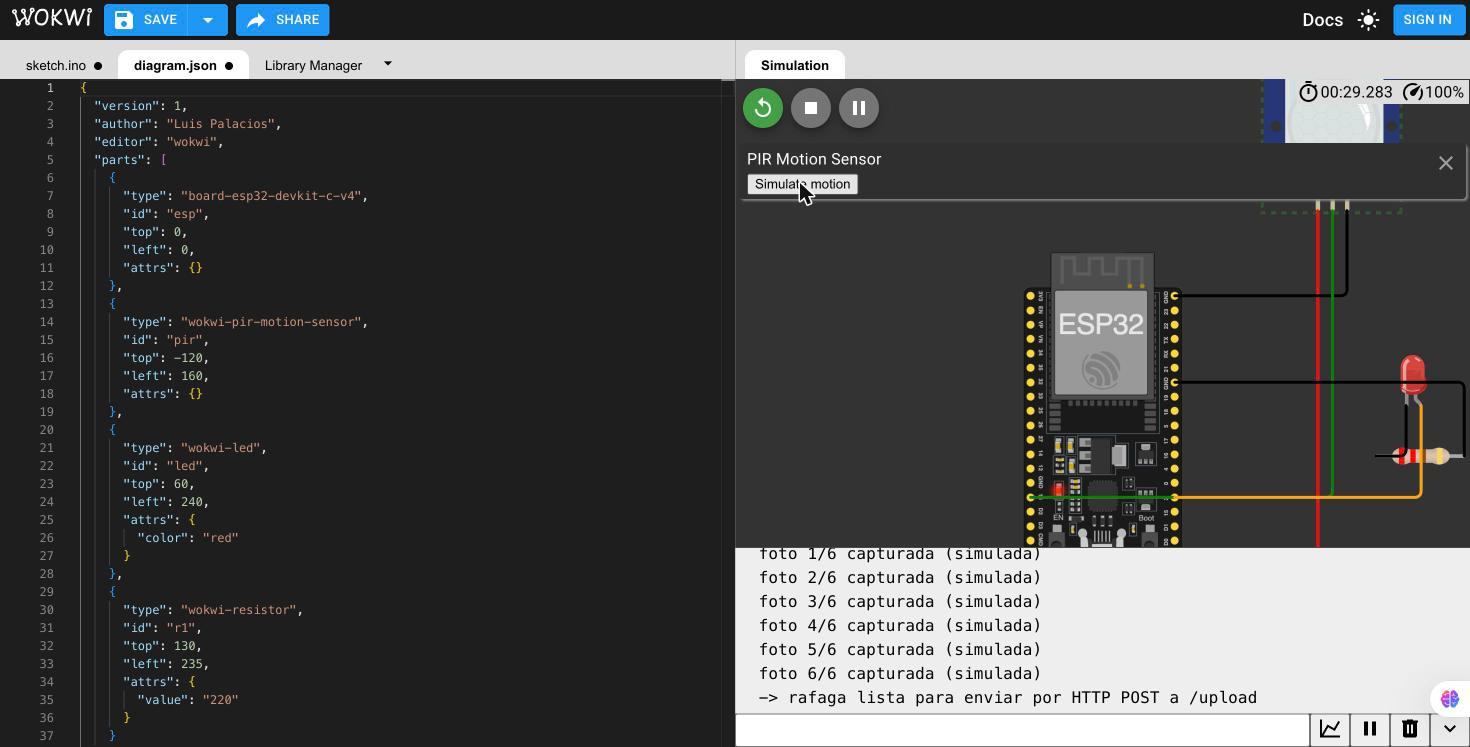
\includegraphics[width=0.85\textwidth]{img/simulacion_wokwi.jpg}
\caption{Simulación en Wokwi: ráfaga de seis fotografías tras un disparo del PIR.}
\label{fig:wokwi}
\end{figure}

%-------------------------------------------------- 5
\section{Avance físico y prueba en hardware real}
\label{sec:fisico}

\subsection{Montaje}

El módulo de cámara es una placa GOOUUU ESP32-S3-CAM v1.5 (microcontrolador ESP32-S3 con cámara OV3660 integrada, 8 MB de PSRAM y dos puertos USB-C). En las pruebas finales se conectó directamente por USB-C al computador, que la alimenta, la programa y le da salida serie (Figura~\ref{fig:montaje}\subref{fig:usb}). Antes se armó un montaje preliminar con la placa sobre una protoboard y cables Dupont hacia un Arduino Uno (Figura~\ref{fig:montaje}\subref{fig:m1} y~\subref{fig:m2}).

\begin{figure}[H]
\centering
\begin{subfigure}[b]{0.31\textwidth}\centering
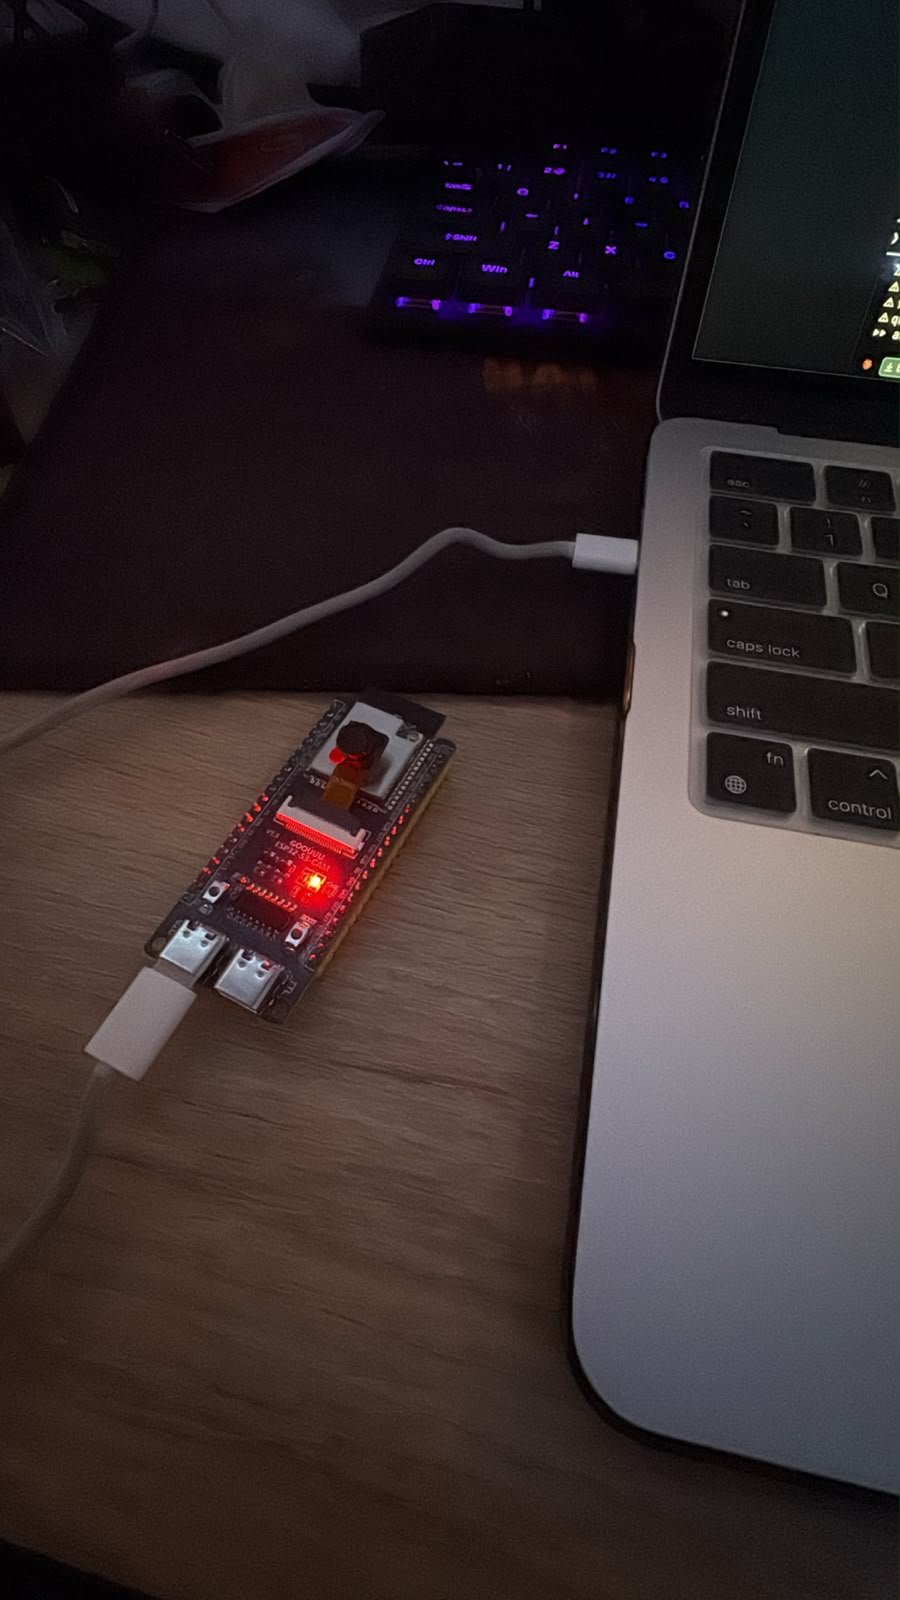
\includegraphics[width=\textwidth]{img/montaje_usb.png}\caption{Conexión USB al computador (pruebas).}\label{fig:usb}
\end{subfigure}\hfill
\begin{subfigure}[b]{0.31\textwidth}\centering
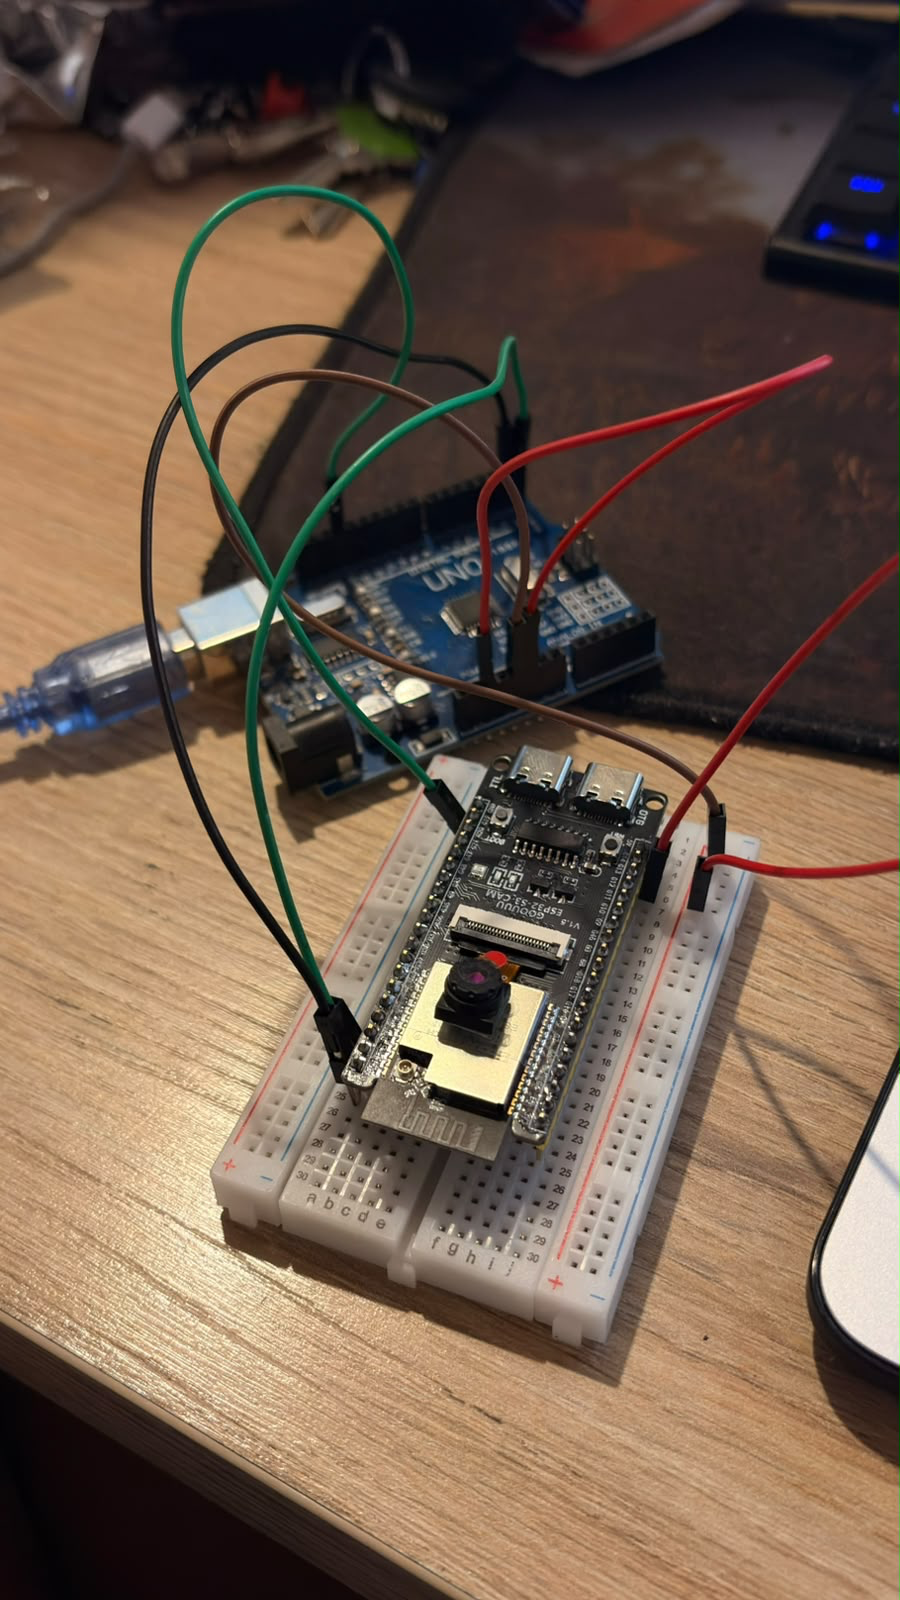
\includegraphics[width=\textwidth]{img/montaje_1.png}\caption{Montaje preliminar con Arduino Uno, vista frontal.}\label{fig:m1}
\end{subfigure}\hfill
\begin{subfigure}[b]{0.31\textwidth}\centering
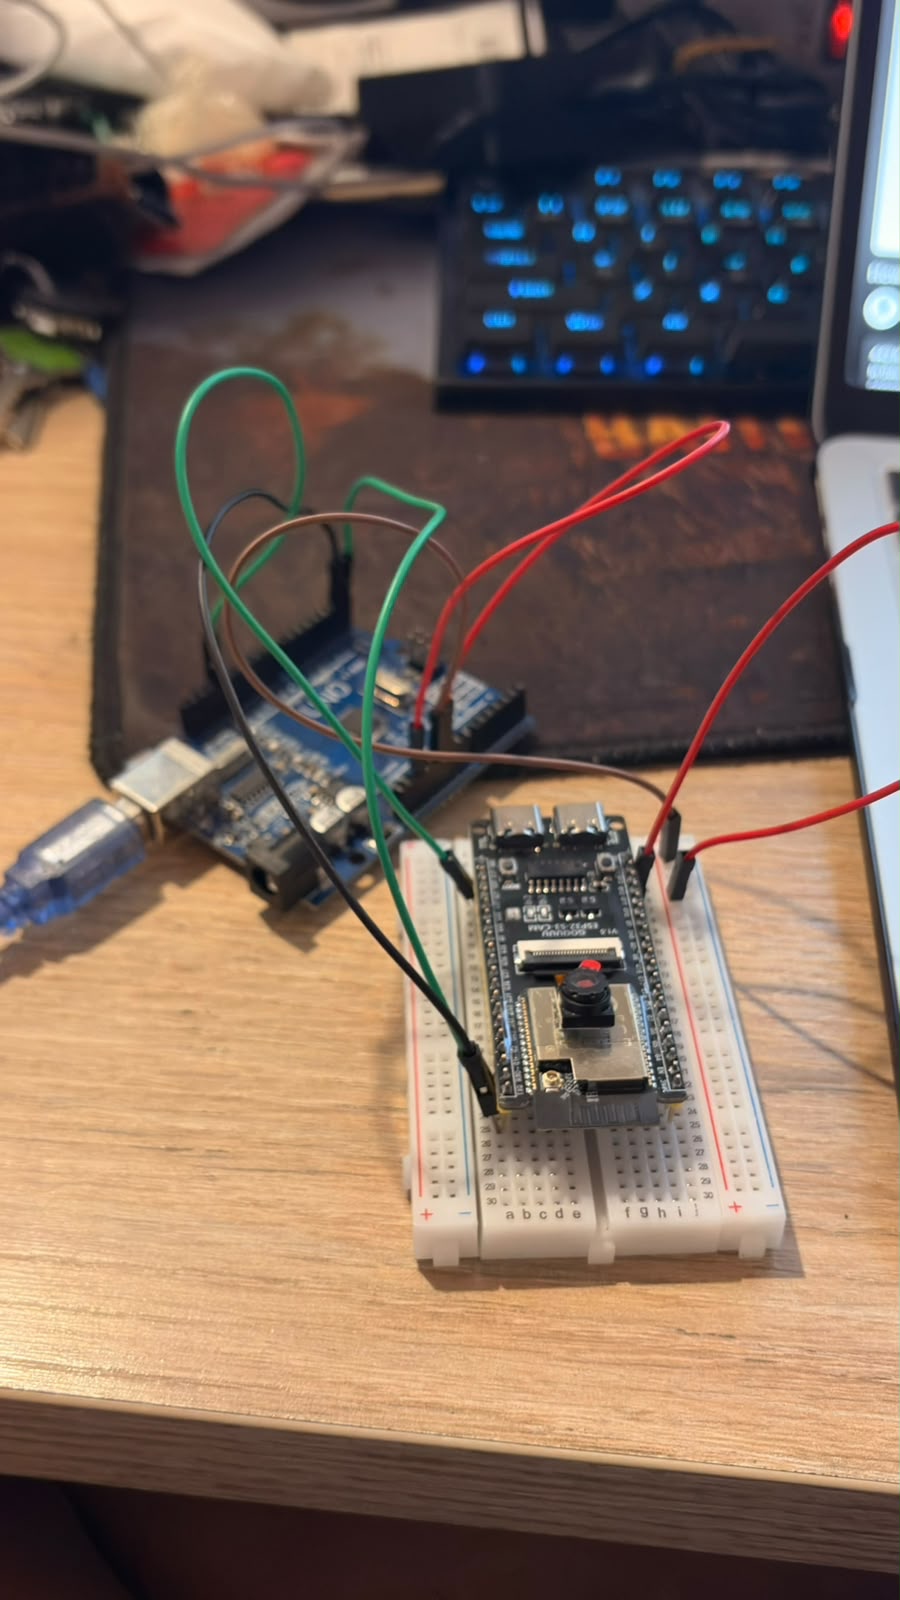
\includegraphics[width=\textwidth]{img/montaje_2.png}\caption{Montaje preliminar, vista lateral.}\label{fig:m2}
\end{subfigure}
\caption{Montaje físico del nodo.}
\label{fig:montaje}
\end{figure}

Para programar esta placa no hace falta el montaje con Arduino, porque cuenta con USB propio. Se conserva como posible configuración para el sitio de instalación: junto al punto de control de plagas, el Arduino Uno y la protoboard permitirían alimentar y concentrar el cableado de periféricos cercanos a la cámara, como el sensor PIR y la iluminación infrarroja. Esta configuración no se ha probado todavía.

\subsection{Firmware del nodo}

El firmware se escribió para el entorno Arduino (paquete \texttt{esp32} 3.3.12), compilado y cargado desde línea de comandos con \texttt{arduino-cli}. La cámara usa la asignación de pines propia de esta placa. Cada disparo captura una ráfaga de seis fotografías en 640$\times$480 píxeles (el tamaño de las escenas de la evaluación), las guarda en la memoria PSRAM y las envía al servidor en una sola petición \texttt{multipart/form-data} al \emph{endpoint} \texttt{/upload}. En esta etapa el disparo se hace con el botón BOOT o con un comando por el puerto serie (\texttt{FOTO}); la integración del PIR queda para la siguiente etapa. Como el sensor OV3660 entrega la imagen invertida, el firmware la corrige por software. El Código~\ref{lst:cam} muestra la configuración de la cámara.

\begin{lstlisting}[language=C++,caption={Configuración de la cámara (fragmento de \texttt{nodo\_plagas.ino}).},label={lst:cam}]
camera_config_t c = {};
c.pin_xclk = 15;  c.pin_pclk = 13;  c.pin_vsync = 6;  c.pin_href = 7;
c.pin_sccb_sda = 4;  c.pin_sccb_scl = 5;
c.xclk_freq_hz = 20000000;
c.pixel_format = PIXFORMAT_JPEG;
c.frame_size   = FRAMESIZE_VGA;        // 640x480
c.jpeg_quality = 12;
c.fb_count     = 2;
c.fb_location  = CAMERA_FB_IN_PSRAM;
esp_err_t err = esp_camera_init(&c);
sensor_t* sen = esp_camera_sensor_get();
sen->set_vflip(sen, 1);               // corrige la imagen invertida del OV3660
\end{lstlisting}

\subsection{Configuración sin credenciales en el código}

Para no incluir la red WiFi ni la dirección del servidor en el código fuente, estos datos se guardan en la memoria flash de la placa (NVS) y se cargan una sola vez por USB con un programa auxiliar (\texttt{configurar\_nodo.py}), que pide la clave por consola sin mostrarla. La placa solo opera en la banda de 2.4 GHz; como los nombres de red no indicaban la frecuencia, la placa escaneó las redes visibles y se identificó la red 2.4 GHz del router comparando su dirección de hardware (BSSID) con la del router al que estaba conectado el computador.

El servidor se localiza por nombre (mDNS, p.\,ej. \texttt{equipo.local}) en cada envío, de modo que el nodo sigue funcionando si el computador cambia de dirección IP (Código~\ref{lst:mdns}).

\begin{lstlisting}[language=C++,caption={Resolución del servidor por nombre en cada envío (fragmento).},label={lst:mdns}]
bool resolverServidor(IPAddress& ip) {
  String h = servidorHost;
  if (h.endsWith(".local")) {
    h.remove(h.length() - 6);
    MDNS.begin("nodo-plagas");
    ip = MDNS.queryHost(h, 3000);          // pregunta en la red local
    return (uint32_t)ip != 0;
  }
  return ip.fromString(h) || WiFi.hostByName(h.c_str(), ip) == 1;
}
\end{lstlisting}

\subsection{Prueba de extremo a extremo}

Con el servidor v2 ejecutándose en el computador, la placa se conectó a la red WiFi, resolvió el servidor por nombre y, al recibir el comando de disparo, capturó una ráfaga de seis fotografías reales y las envió. El servidor las recibió y respondió con código 200 y estado \texttt{evaluado} (Código~\ref{lst:serie}). La Figura~\ref{fig:real} muestra las seis fotografías de esa ráfaga, que se entregan como evidencia junto con el registro de la prueba.

\begin{lstlisting}[caption={Salida serie de la placa durante el disparo (prueba real).},label={lst:serie}]
[PSRAM] ok (8388608 bytes)
[CAM] camara lista
[WiFi] conectando....... ok, IP 192.168.0.30
[DISPARO] capturando rafaga...
  foto 1/6 (28632 bytes)
  ...
  foto 6/6 (25295 bytes)
[HTTP] servidor equipo.local -> 192.168.0.26
[HTTP] HTTP/1.1 200 OK
[HTTP] respuesta: {"alerta":true,"estado":"evaluado",
                   "eventos":[ ...6 regiones... ]}
\end{lstlisting}

\begin{figure}[H]
\centering
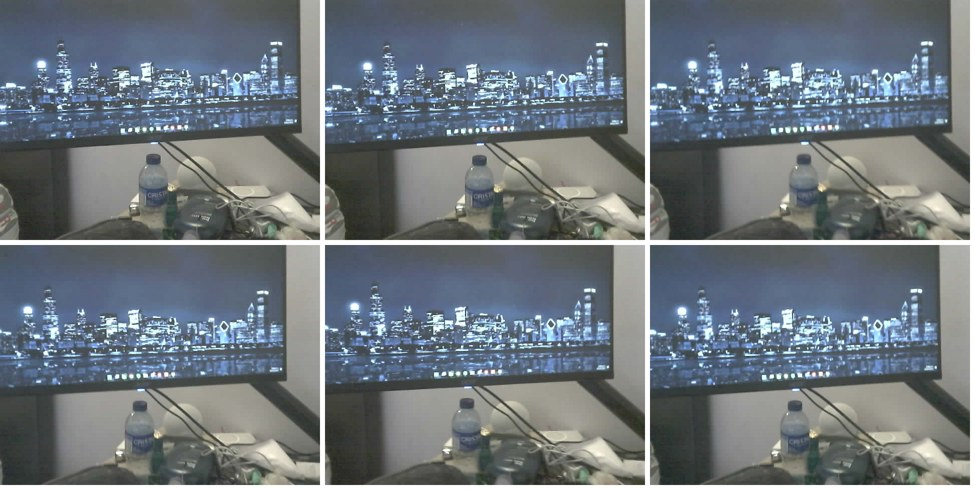
\includegraphics[width=0.85\textwidth]{img/rafaga_real.jpg}
\caption{Ráfaga de seis fotografías reales (640$\times$480) capturadas por la cámara y recibidas por el servidor.}
\label{fig:real}
\end{figure}

La escena fotografiada contiene un monitor y una botella, sin plagas ni objetos en movimiento. Aun así, el servidor marcó seis regiones de entre 152 y 433 píxeles como posible actividad (Figura~\ref{fig:snap}). Se trata de falsos positivos: las regiones coinciden con zonas de alto contraste, como las luces del monitor, su reflejo y el borde de la botella. No se verificó la causa; es probable que se deba al ruido del sensor y a una leve vibración, que son más intensos en la cámara real que en las escenas sintéticas usadas para la evaluación (Sección~\ref{sec:eval}). Este resultado confirma que el flujo completo funciona, y que los umbrales del detector deben calibrarse con escenas reales antes de afirmar un desempeño con la cámara.

\begin{figure}[H]
\centering
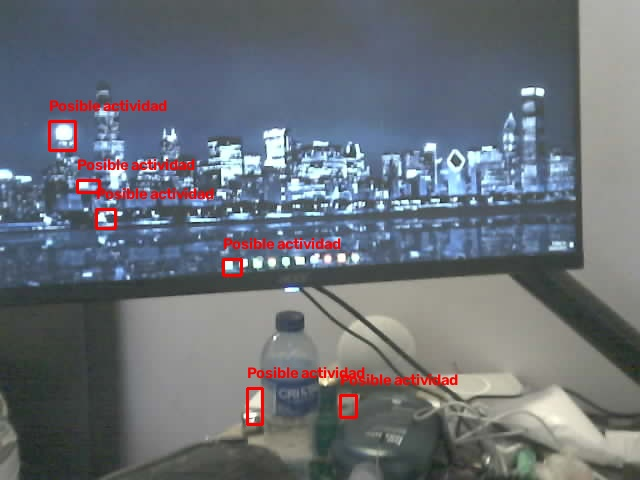
\includegraphics[width=0.55\textwidth]{img/snapshot_real.jpg}
\caption{Imagen anotada por el servidor: las seis regiones marcadas son falsos positivos (escena sin plagas).}
\label{fig:snap}
\end{figure}

Esta prueba no se hizo con objetos ni plagas reales, ni con el sensor PIR conectado.

%-------------------------------------------------- 6
\section{Limitaciones}

\begin{itemize}
\item La evaluación cuantitativa se hizo con imágenes sintéticas. En la prueba con la cámara real, el detector marcó falsos positivos en una escena sin plagas, por lo que los umbrales (área de 150 a 8000 px, sensibilidad del sustractor) deben calibrarse con escenas reales, y el ruido real del sensor es mayor que el simulado.
\item El sensor PIR aún no está integrado al firmware real; el disparo es por botón o por comando serie. El PIR detecta cambios de radiación infrarroja (calor), no insectos, por lo que un insecto pequeño podría no activarlo. Esto debe evaluarse con el hardware.
\item Con el PIR, una plaga ya estaría a la vista durante toda la ráfaga y el modelo podría aprenderla como fondo. Un diseño más robusto separa las fotografías de fondo, tomadas periódicamente, de la fotografía del disparo; está pendiente de implementar y evaluar.
\item La placa solo opera en 2.4 GHz y requiere una configuración inicial por USB para registrar la red WiFi.
\item Las alertas locales o remotas y la operación con varios nodos reales no están implementadas; el panel web es solo un prototipo de consulta.
\item La instalación de cámaras en zonas de trabajo plantea consideraciones de privacidad del personal.
\end{itemize}

%-------------------------------------------------- 7
\section{Conclusiones}

Se cuenta con un servidor de procesamiento verificado mediante 17 pruebas automáticas, cuya segunda versión corrige las limitaciones de la primera (modelo de fondo por zona, ráfagas, calentamiento y validación de entradas), con una simulación de la lógica del nodo y con un nodo físico funcional: la placa captura ráfagas reales y las envía por WiFi al servidor, que las procesa. La primera prueba con la cámara real mostró falsos positivos en una escena sin plagas, lo que hace necesaria la calibración. La evaluación con escenas sintéticas respalda el diseño, aunque no sustituye la validación con escenas reales. Quedan pendientes la integración del PIR, la calibración de los umbrales con objetos reales y el rediseño de la captura de fondo descrito en las limitaciones.

\end{document}
